\documentclass[12pt,tikz,border=10pt]{standalone}
\usetikzlibrary{arrows.meta, positioning, calc, fit}
\usepackage{amsmath}
\usepackage{amssymb}

\begin{document}
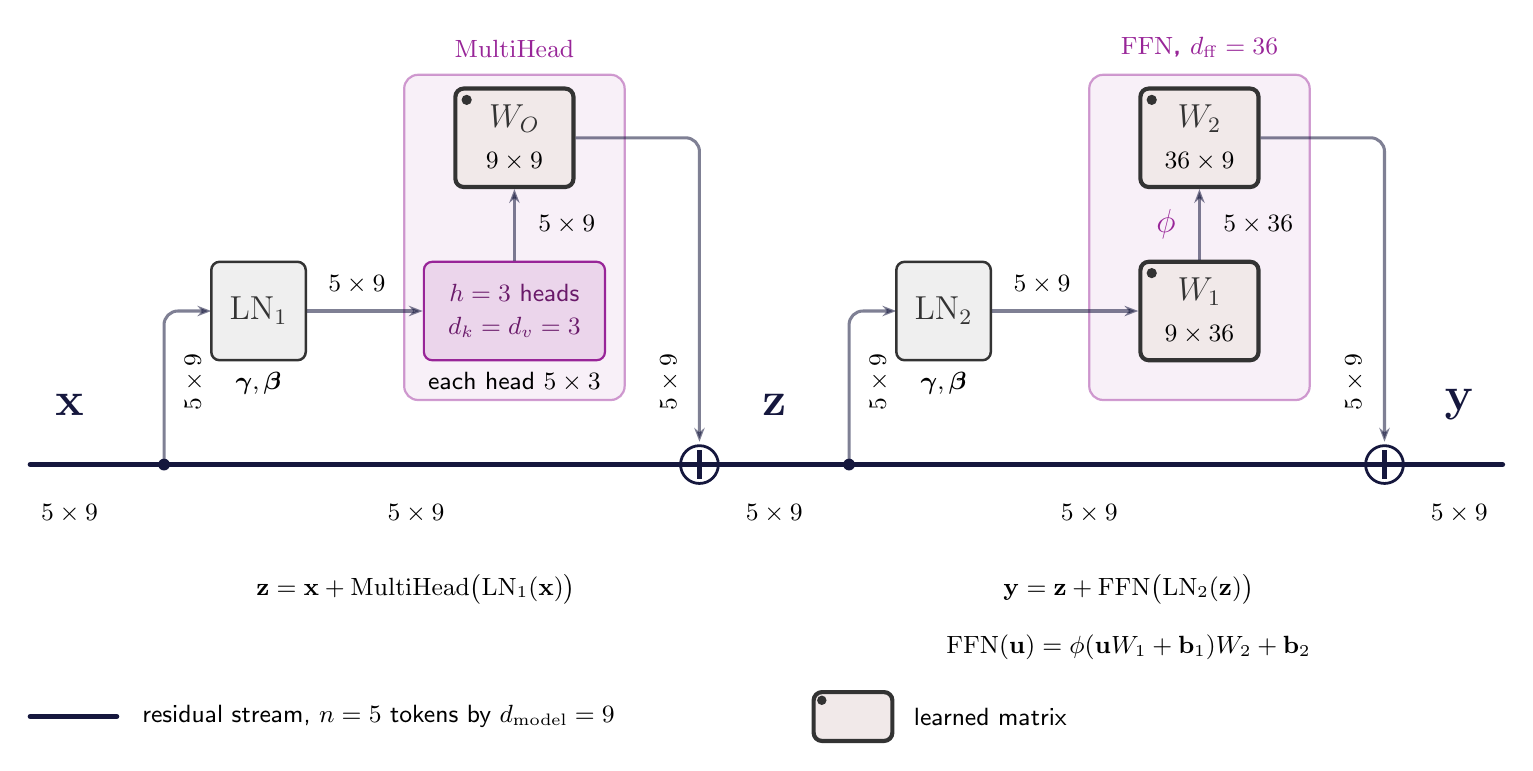
\begin{tikzpicture}[
    every node/.style={font=\sffamily},
]

\definecolor{c1}{HTML}{15173D}
\definecolor{c2}{HTML}{982598}
\definecolor{c3}{HTML}{E491C9}
\definecolor{c4}{HTML}{F1E9E9}
\definecolor{axiscolor}{HTML}{333333}
\definecolor{labelcolor}{HTML}{000000}

% ================================================================
% VISUAL GRAMMAR (shared across section 10)
%   stream        : c1, 2.4pt, y = 0, unbroken end to end, nothing on it
%   branch        : c1 at opacity 0.55, leaves the stream and rejoins it
%   sublayer box  : c2 panel, hanging OFF the stream (as residual_stream)
%   LN            : neutral grey box, no corner dot, gamma/beta underneath
%   learned matrix: thick axiscolor outline + corner dot, shape on line 2
%   (+)           : r = 0.24 circle, white fill, c1 1.0pt; the stream is
%                   the horizontal bar, re-stroked across the circle
%
% VERTICAL PLAN  (the panels are stacked internally, to buy height)
%   panel      0.88 .. 4.95      title (anchor south) 5.05
%   upper box  3.525 .. 4.775    centre yU = 4.15   (W_O / W_2)
%   arrow gap  2.575 .. 3.525    edge labels at 3.05
%   lower box  1.325 .. 2.575    centre yL = 1.95   (heads / W_1)
%   sub-labels (anchor north)    1.30
%   stream     0                 symbols 0.72, stream shapes -0.62
%   equations -1.55, FFN expansion -2.25, legend -3.15
%
% HORIZONTAL PLAN, per sublayer with tap at T:
%   LN centre T+1.20 (w 1.2) | shape label T+2.45 | panel T+3.05..T+5.85
%   inner boxes centre T+4.45 | add T+6.80
%   T1 = 0.85  add1 = 7.65   T2 = 9.55  add2 = 16.35
%   x -0.35 | z 8.60 | y 17.30 | stream -0.85 .. 17.85
% Riser shape labels are rotated and sit on the INSIDE of each sublayer,
% so they are never near the x, z, y glyphs.
% ================================================================

\def\yL{1.95}
\def\yU{4.15}
\def\pbot{0.82}
\def\ptop{4.95}
\def\ysub{1.30}
\def\ymid{3.05}

\tikzset{
  stream/.style={c1, line width=1.8pt, line cap=round},
  branch/.style={-{Stealth[length=5pt]}, c1, opacity=0.55, line width=1.1pt,
                 rounded corners=5pt},
  panel/.style={draw=c2, line width=0.8pt, draw opacity=0.45, fill=c2,
                fill opacity=0.07, rounded corners=5pt},
  ptitle/.style={font=\sffamily\small\bfseries, text=c2, anchor=south},
  norm/.style={draw=axiscolor, line width=0.9pt, fill=axiscolor,
               fill opacity=0.08, text opacity=1, rounded corners=3pt,
               minimum width=1.2cm, minimum height=1.25cm,
               font=\sffamily\large, text=axiscolor},
  inner/.style={draw=c2, line width=0.8pt, fill=c2, fill opacity=0.13,
                text opacity=1, rounded corners=3pt, minimum height=1.25cm,
                minimum width=2.3cm, font=\sffamily\small,
                text=c2!70!black, align=center},
  learn/.style={draw=axiscolor, line width=1.5pt, fill=c4, rounded corners=3pt,
                minimum width=1.5cm, minimum height=1.25cm, align=center,
                font=\sffamily\large, text=axiscolor},
  shp/.style={font=\sffamily\small, text=black},
  sub/.style={font=\sffamily\small, text=black, anchor=north},
  sym/.style={font=\sffamily\LARGE, text=c1},
  eq/.style={font=\sffamily\small, text=black},
}

\newcommand{\dotmark}[1]{\fill[axiscolor] ($(#1.north west)+(0.17,-0.17)$)
    circle (0.065);}
\newcommand{\wshape}[1]{\\[1pt]{\small\color{black}#1}}

% the stream itself is the horizontal bar of the plus: white circle, then
% the stream re-stroked straight across it, then the vertical stroke only
\newcommand{\plusnode}[1]{%
  \draw[fill=white, draw=c1, line width=1.0pt] (#1, 0) circle (0.24);
  \draw[c1, line width=1.8pt] (#1-0.24, 0) -- (#1+0.24, 0);
  \draw[c1, line width=1.8pt] (#1, -0.18) -- (#1, 0.18);}

% ---------------------------------------------------------------- stream
\draw[stream] (-0.85, 0) -- (17.85, 0);

\node[sym] at (-0.35, 0.76) {$\mathbf{x}$};
\node[sym] at (8.60, 0.76) {$\mathbf{z}$};
\node[sym] at (17.30, 0.76) {$\mathbf{y}$};
\foreach \x in {-0.35, 4.05, 8.60, 12.60, 17.30} {
    \node[shp] at (\x, -0.62) {$5 \times 9$};
}

% ================================================================
% sublayer 1: multi-head attention   (tap 0.85, add 7.65)
% ================================================================
\fill[c1] (0.85, 0) circle (0.075);
\draw[branch] (0.85, 0) -- (0.85, \yL) -- (1.45, \yL);
\node[shp, rotate=90, anchor=north] at (0.99, 1.05) {$5 \times 9$};

\node[norm] (ln1) at (2.05, \yL) {$\mathrm{LN}_1$};
\node[sub] at (2.05, \ysub) {$\boldsymbol{\gamma}, \boldsymbol{\beta}$};

\draw[panel] (3.90, \pbot) rectangle (6.70, \ptop);
\node[ptitle] at (5.30, \ptop+0.10) {$\mathrm{MultiHead}$};

\node[inner] (hd) at (5.30, \yL) {$h = 3$ heads\\[1pt] $d_k = d_v = 3$};
\node[sub] at (5.30, \ysub) {each head $5 \times 3$};

\node[learn] (wo) at (5.30, \yU) {$W_O$\wshape{$9 \times 9$}};  \dotmark{wo}

\draw[branch] (ln1.east) -- (hd.west);
\node[shp, anchor=south] at (3.30, 2.04) {$5 \times 9$};

\draw[branch] (hd.north) -- (wo.south);
\node[shp, anchor=west] at (5.48, \ymid) {$5 \times 9$};

\draw[branch] (wo.east) -- (7.65, \yU) -- (7.65, 0.29);
\node[shp, rotate=90, anchor=south] at (7.51, 1.05) {$5 \times 9$};

% ================================================================
% sublayer 2: feed-forward           (tap 9.55, add 16.35)
% ================================================================
\fill[c1] (9.55, 0) circle (0.075);
\draw[branch] (9.55, 0) -- (9.55, \yL) -- (10.15, \yL);
\node[shp, rotate=90, anchor=north] at (9.69, 1.05) {$5 \times 9$};

\node[norm] (ln2) at (10.75, \yL) {$\mathrm{LN}_2$};
\node[sub] at (10.75, \ysub) {$\boldsymbol{\gamma}, \boldsymbol{\beta}$};

\draw[panel] (12.60, \pbot) rectangle (15.40, \ptop);
\node[ptitle] at (14.00, \ptop+0.10) {$\mathrm{FFN}$, $d_{\mathrm{ff}} = 36$};

\node[learn] (w1) at (14.00, \yL) {$W_1$\wshape{$9 \times 36$}};  \dotmark{w1}
\node[learn] (w2) at (14.00, \yU) {$W_2$\wshape{$36 \times 9$}};  \dotmark{w2}
\draw[branch] (ln2.east) -- (w1.west);
\node[shp, anchor=south] at (12.00, 2.04) {$5 \times 9$};

\draw[branch] (w1.north) -- (w2.south);
\node[shp, anchor=west] at (14.18, \ymid) {$5 \times 36$};
\node[anchor=east, text=c2, font=\sffamily\large] at (13.82, \ymid) {$\phi$};

\draw[branch] (w2.east) -- (16.35, \yU) -- (16.35, 0.29);
\node[shp, rotate=90, anchor=south] at (16.21, 1.05) {$5 \times 9$};

% ---------------------------------------------------------------- the adds
\plusnode{7.65}
\plusnode{16.35}

% ---------------------------------------------------------------- equations
\node[eq] at (4.05, -1.58)
    {$\mathbf{z} = \mathbf{x} + \mathrm{MultiHead}\bigl(\mathrm{LN}_1(\mathbf{x})\bigr)$};
\node[eq] at (13.10, -1.58)
    {$\mathbf{y} = \mathbf{z} + \mathrm{FFN}\bigl(\mathrm{LN}_2(\mathbf{z})\bigr)$};
\node[eq] at (13.10, -2.32)
    {$\mathrm{FFN}(\mathbf{u}) = \phi(\mathbf{u} W_1 + \mathbf{b}_1) W_2 + \mathbf{b}_2$};

% ---------------------------------------------------------------- legend
\draw[stream] (-0.85, -3.20) -- (0.25, -3.20);
\node[shp, anchor=west, text=black] at (0.45, -3.20)
    {residual stream, $n = 5$ tokens by $d_{\mathrm{model}} = 9$};

\node[learn, minimum width=1.0cm, minimum height=0.62cm] (lg)
    at (9.60, -3.20) {\phantom{$W$}};
\fill[axiscolor] ($(lg.north west)+(0.13,-0.13)$) circle (0.06);
\node[shp, anchor=west, text=black] at (10.25, -3.20) {learned matrix};

\end{tikzpicture}
\end{document}
